\documentclass{article}
\usepackage{pdfpages}

% Importeer configuratie-instellingen
\RequirePackage{../../LaTeX/config}

% Begin van het document
\begin{document}

% FMW-specifiek titelblad voordat het examen begint
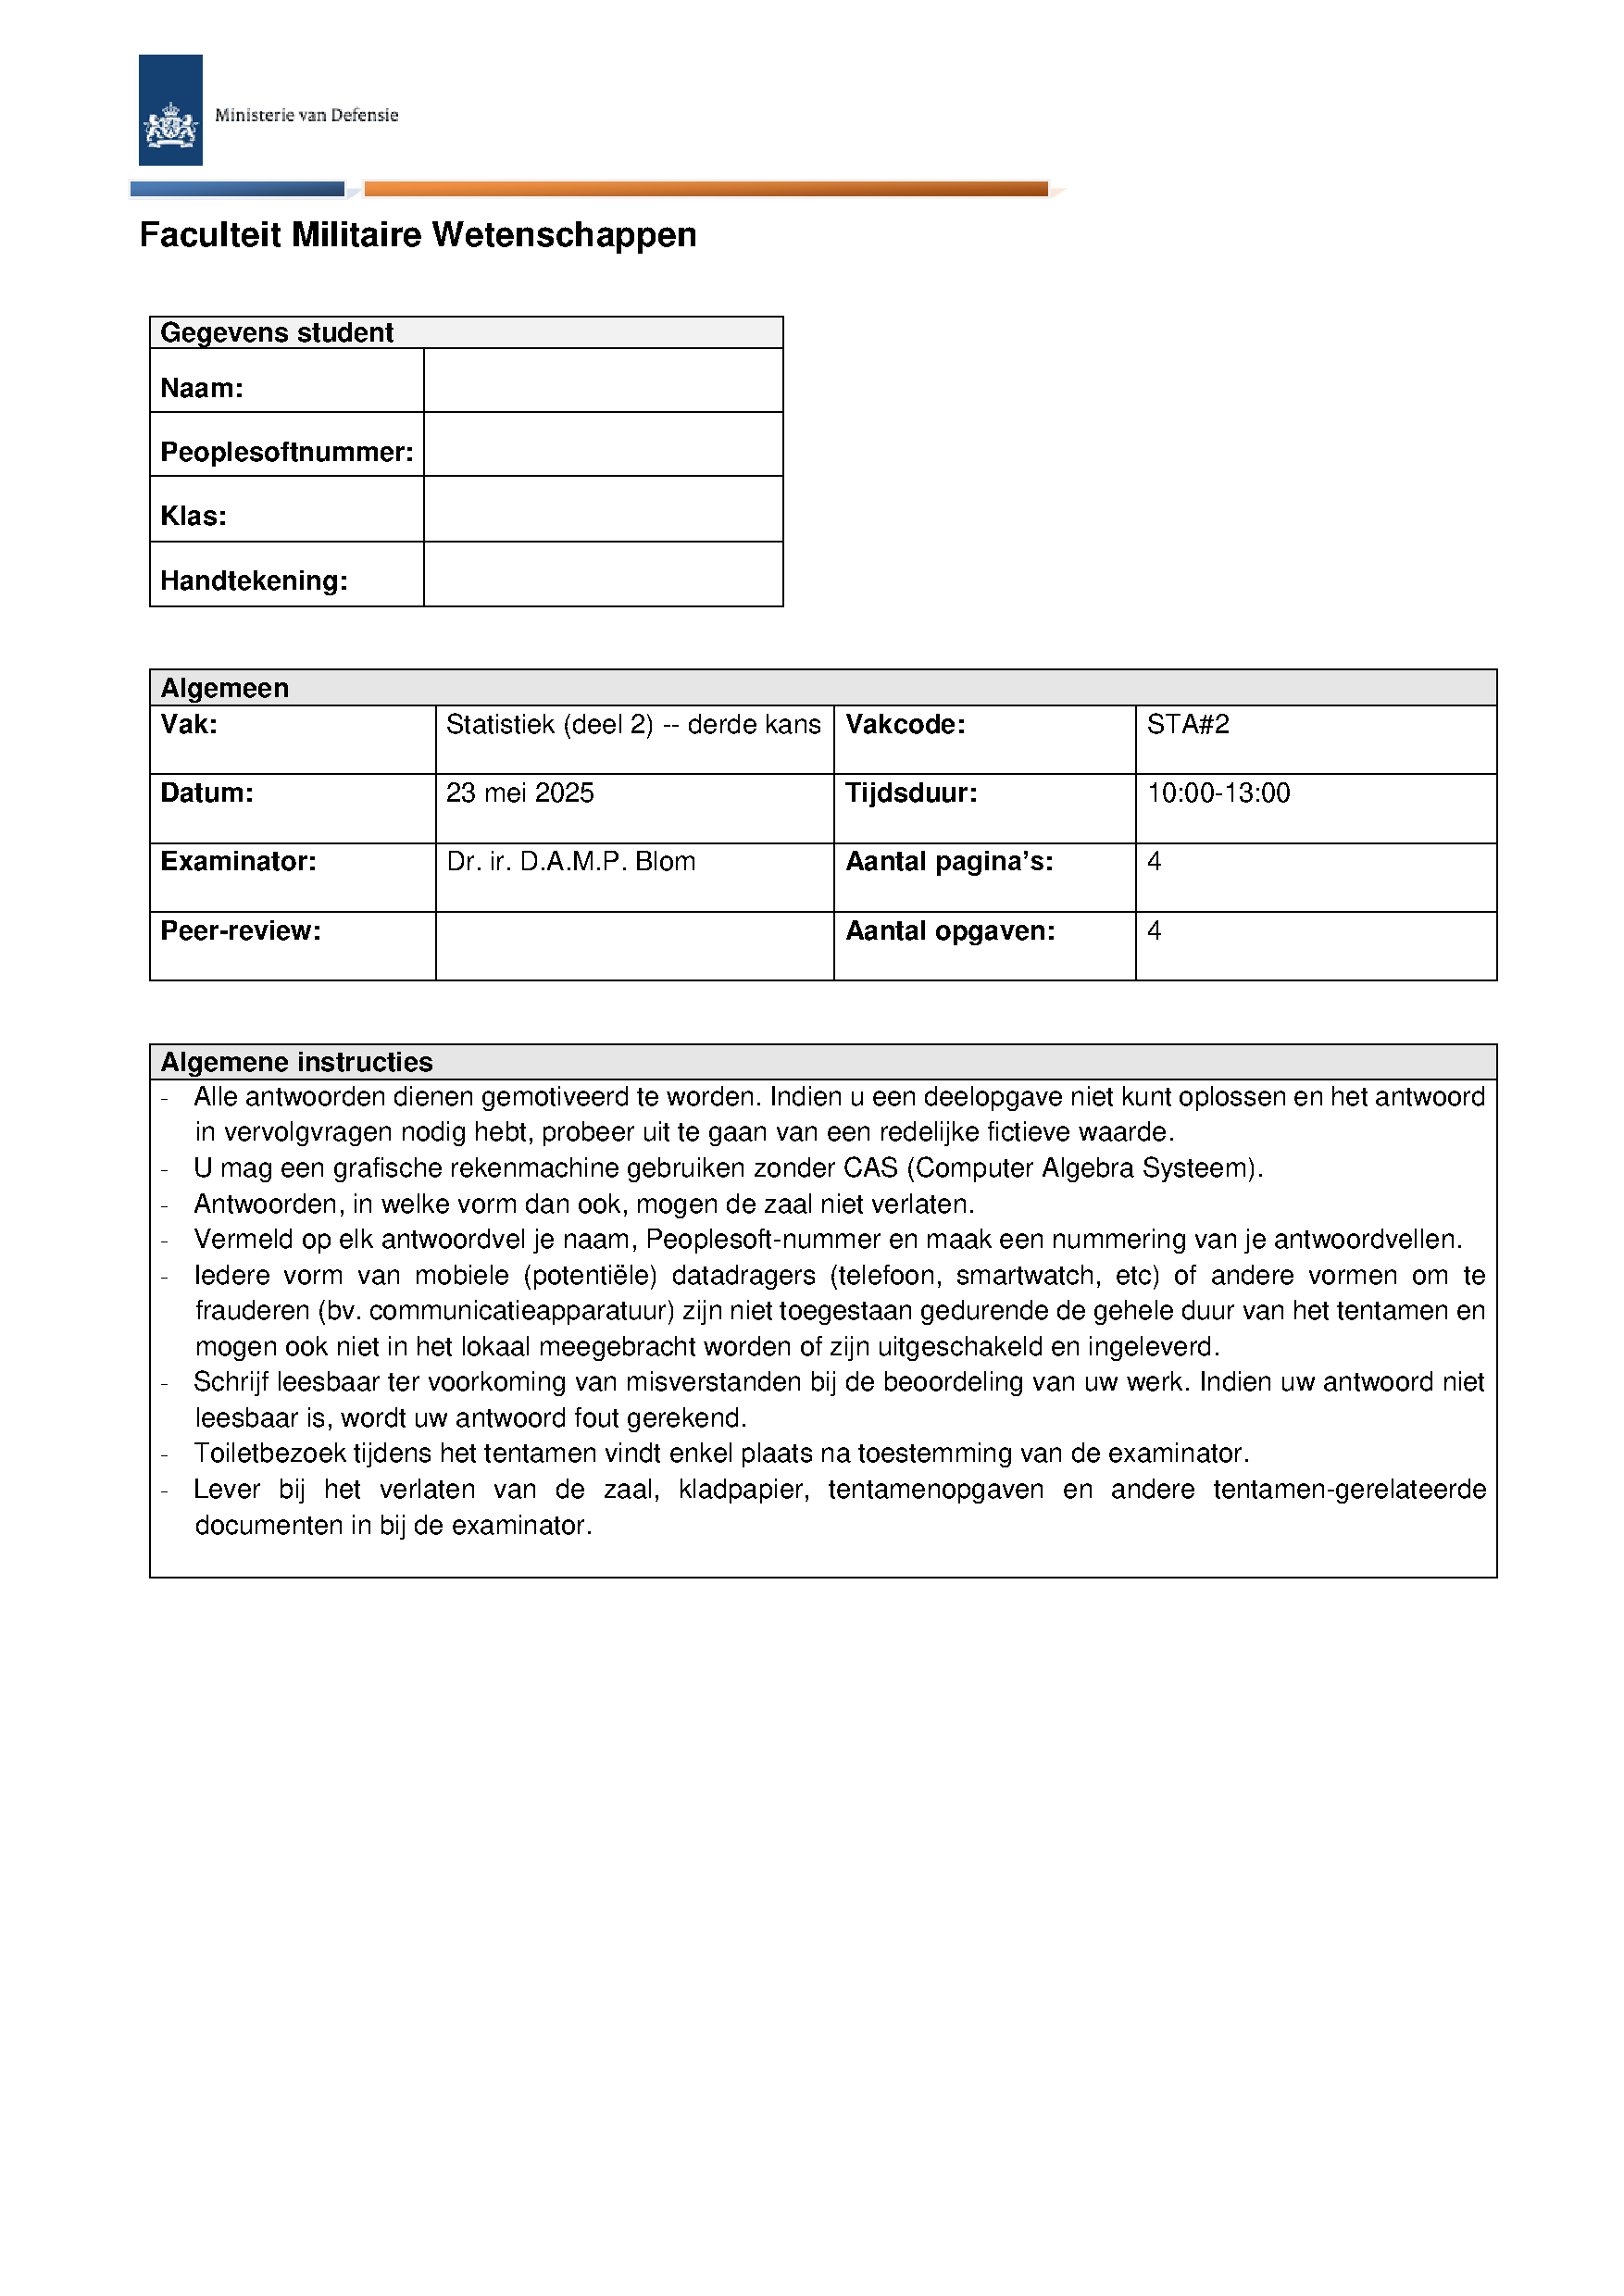
\includepdf{../../Python/FMW_titelblad_20250523.pdf}

\title{Tentamen statistiek}
\author{Nederlandse Defensie Academie}
\date{\today}
\maketitle

% Include questions from external files
\section*{Vragen}

\begin{question}{22}{
    Een onderzoeksteam van het Maritime Warfare Center (MWC) onderzoekt de signaalsterkte (in decibel) van sonarpulsen die worden gereflecteerd door een nieuw type onderzeeboot.
    Het huidige ontwerp heeft een gemiddelde gereflecteerde signaalsterkte van $\mu = 65$ decibel.

    Het MWC wil toetsen of het nieuw ontwerp de detecteerbaarheid reduceert, oftewel dat de gereflecteerde signaalsterkte significant lager ligt bij het nieuwe ontwerp.
    In een steekproef van tien onafhankelijke metingen is bij het nieuwe ontwerp de gereflecteerde signaalsterkte in decibel gemeten met gemiddelde $63,75$ decibel en standaardafwijking $s = 0,78$.
    Je mag aannemen dat de signaalsterktes normaal verdeeld zijn met onbekende standaardafwijking $\sigma$.
    
    Gebruik voor de hypothesetoets een significantieniveau van $\alpha=0,05$.
}
    \subquestion{4}{
       Definieer de nulhypothese en de alternatieve hypothese van de hypothesetoets.
       Verklaar het gekozen type (tweezijdig, linkszijdig of rechtszijdig) van de toets.
    }
    \solution{
        Aangezien we willen toetsen of de gemiddelde gereflecteerde signaalsterkte significant lager ligt dan $\mu = 65$, kunnen we de hypothesetoets als volgt defini\"eren:
        \begin{align*}
            H_0&: \mu \ge 65 \quad \text{(geen significante vermindering)} \rubric{2} \\
            H_1&: \mu < 65 \quad \text{(wel een significante vermindering)} \rubric{1}
        \end{align*}
        Dit is een linkszijdige toets, omdat de nulhypothese uitgaat van een status-quo (geen verbetering) en de alternatieve hypothese juist wel een verbetering aanduidt.
         \rubric{1}
    }
    
    \subquestion{4}{
       Voer de bijbehorende hypothesetoets uit met behulp van het kritieke gebied.
    }
    \solution{
        Aangezien de steekproefgrootte $n = 10$ kleiner is dan $30$ en de standaardafwijking $\sigma$ onbekend is, moeten we de $t$-verdeling gebruiken. \rubric{1}
        Deze $t$-verdeling heeft $\text{df}=n-1=9$ vrijheidsgraden.\rubric{1}

        De toetsingsgrootheid van onze hypothesetoets is gelijk aan
        \begin{align*}
            t = \frac{
        \end{align*}
        We willen een kritiek gebied bepalen voor het populatiegemiddelde $\mu$ met significantieniveau $\alpha = 0,05$.
        Dit doen we aan de hand van de $t$-waarde
        \[
            t = \invt(\text{area}=1 - \alpha; \text{df}=n-1) = \invt(\text{area}=0.95; \text{df}=9) = 1.8331. \rubric{2}
        \]
        Since the hypothesis is left-tailed, the critical region is of the form $(-\infty, g]$. \rubric{1}
        In particular, we can compute the boundary $g$ as follows
        \begin{align*}
            g   &= \mu - t \cdot \frac{s}{\sqrt{n}} \\
                &= 65 - 1.8331 \cdot \frac{0.7792}{\sqrt{10}} \\
                &\approx 64.5483 \rubric{2}
        \end{align*}  
        
        The critical region is therefore be given by $(-\infty; 64.5483]$.\rubric{1}
        The sample mean (test statistic) $\overline{x}=63.75$ lies in the critical region, hence we reject the null hypothesis $H_0$.
        Based on the selected sample, there is sufficient evidence to believe that the new stealth design indeed reduces detectability.\rubric{1}
        }

    
    \subquestion{4}{Calculate the probability of a Type-II error $\beta$ if the true reflected signal strength is actually normally distributed with $\mu = 64.5$ en $\sigma=0.8$ dB (for a single observation).}

    \solution{
        We computed in the previous subquestion the critical region, which was equal to $(-\infty; 64.5483]$.
        Therefore, we need to compute the probability that given $\mu=64$ en $\sigma=0.8$, we get a value inside the acceptable region. \rubric{1}

        In other words:
        \begin{align*}
            \beta   &= P(\overline{X} < 64.5483 \mid \mu = 64.5) \\
                    &= \normalcdf(\text{lower}=-10^{99}; \text{upper}=64.5483; \mu=64.5; \sigma=\frac{0.8}{\sqrt{10}}) \\
                    &\approx 0.5757 \rubric{2}
        \end{align*}

        So, $\beta \approx 0.5757$: a $57,57\%$ chance of accepting the null hypothesis while it is incorrect in reality. \rubric{1}
    }
\end{question}
\begin{question}{30}{
    Een luchtmachteenheid is een nieuw type radar aan het testen voor het detecteren van vijandelijke drones.
    Fabrikant Thales claimt dat de radar een succeskans van \SI{70}{\percent} heeft om een drone te detecteren (onafhankelijk van andere drones).
    Om deze claim te testen, worden er $1000$ onafhankelijke tests uitgevoerd. In elke test worden vier drones op het systeem afgestuurd en geteld hoeveel van de vier drones gedetecteerd worden.
    De gegevens zijn weergegeven in onderstaande frequentietabel:
    \begin{center}
        \renewcommand{\arraystretch}{0.75}
        \begin{tabular}{cc}
            \toprule
                \textbf{Aantal drones} & \textbf{Frequentie} \\
            \midrule
                $0$ & $15$ \\
                $1$ & $105$ \\
                $2$ & $290$ \\
                $3$ & $360$ \\
                $4$ & $230$ \\
            \bottomrule
        \end{tabular}
    \end{center}

    Om de claim van de fabrikant te toetsen, wordt een chikwadraat aanpassingstoets uitgevoerd.
}
\vspace{-1cm}
    \subquestion{4}{
        Welke kansverdeling volgt het aantal gedetecteerde drones in één enkele test met een radar?
        Geef daarnaast specifieke waardes van de bijbehorende parameters.
    }

    \solution{
        Laat $X$ het aantal gedetecteerde drones zijn in één enkele test met de radar.
        Omdat we een ``aantal successen'' (detecties) tellen uit een eindig aantal onafhankelijke Bernoulli-experimenten (aantal drones), betreft het een binomiale kansverdeling. \rubric{2}
        
        Het aantal Bernoulli-experimenten $n = 4$, want er doen vier drones mee per test.\rubric{1}

        Verder is de succeskans $p = 0.7$ (\SI{70}{\percent} detectiekans) per drone. \rubric{1}
    
        {
            \itshape Noot: de waarde van $n$ is NIET gelijk aan $1000$. Dit getal geeft alleen aan hoe vaak een realisatie van een Binomiaal$(n=4,p=0.7)$ verdeelde kansvariabele wordt gemeten.
        }
    }

    \subquestion{4}{
        Formuleer de nulhypothese $H_0$ en de alternatieve $H_1$ van deze hypothesetoets.
        Wat zou in deze context de betekenis zijn van het verwerpen van de nulhypothese?
    }

    \solution{
        De nulhypothese $H_0$ en de alternatieve hypothesetoets $H_1$ kunnen als volgt worden geformuleerd:
        \begin{description}
            \item[$H_0$:] het aantal gedetecteerde drones $X$ volgt een binomiale verdeling met parameters $n = 4$ en $p = 0.7$ \rubric{1}
            \item[$H_1$:] het aantal gedetecteerde drones $X$ volgt NIET een binomiale verdeling met parameters $n = 4$ en $p = 0.7$ \rubric{1}
        \end{description}
        Het verwerpen van de nulhypothese $H_0$ betekent in dit geval dat $X$ niet binomiaal verdeeld met parameters $n = 4$ en $p = 0.7$.\rubric{1}
        Het is echter nog steeds mogelijk dat $X$ binomiaal verdeeld is, maar dan moet gelden dat de succeskans $p \neq 0.7$.\rubric{1}
    }

    \subquestion{3}{
        Bereken de verwachte (``expected'') frequenties van het aantal gedetecteerde drones uitgaande van de nulhypothese $H_0$.
    }
    \solution{
        Om de verwachte frequenties te bepalen, moeten we gebruik maken van het feit dat er $1000$ onafhankelijke tests zijn uitgevoerd.
        Onder de nulhypothese $H_0$ is het aantal gedetecteerde drones $X$ binomiaal verdeeld met parameters $n = 4$ en $p = 0.7$. \rubric{1}
        
        {\small
            \begin{center}
                \renewcommand{\arraystretch}{1.25}
                \begin{tabular}{ccc}
                    \toprule
                        \textbf{Aantal drones} & \textbf{Observed} & \textbf{Expected} \\
                    \midrule
                        $0$ & $15$  & $1000 \cdot \binompdf(n=4, p=0.7, k=0) = 8.1$   \\
                        $1$ & $105$ & $1000 \cdot \binompdf(n=4, p=0.7, k=1) = 75.6$  \\
                        $2$ & $290$ & $1000 \cdot \binompdf(n=4, p=0.7, k=2) = 264.6$ \\
                        $3$ & $360$ & $1000 \cdot \binompdf(n=4, p=0.7, k=3) = 411.6$ \\
                        $4$ & $230$ & $1000 \cdot \binompdf(n=4, p=0.7, k=4) = 240.1$ \rubric{2} \\
                    \bottomrule
                \end{tabular}
            \end{center}
        }
    }

    \subquestion{6}{
        Bereken de toetsingsgrootheid en de $p$-waarde op basis van de gegeven frequenties.
    }
    \solution{
        We berekenen de toetsingsgrootheid $\chi^2$ als volgt:

        \begin{align*}
            \chi^2 &= \frac{(O_{0} - E_{0})^2}{E_{0}} + \frac{(O_{1} - E_{1})^2}{E_{1}} + \ldots + \frac{(O_{4} - E_{4})^2}{E_{4}}\\
                    &= \frac{(15 - 8.1)^2}{8.1} + \frac{(105 - 75.6)^2}{75.6} + \ldots + \frac{(230 - 240.1)^2}{240.1}\\
                    &\approx 26.643 
        \end{align*}
    
        De theoretische toetsingsgrootheid $X^2$ volgt onder de nulhypothese een $\chi^2$-verdeling met $\text{df}= \#\textrm{categorieën} - 1 = 4$ vrijheidsgraden.
        De $p$-waarde behorende bij onze toetsingsgrootheid is daarom gelijk aan        \begin{align*}
            p = P(\chi^2 > 26.643) &= \chi^2\text{cdf}(\text{lower}=26.643; \text{upper}=10^{99}; \text{df}=4) \\
                                             &\approx 0.   
        \end{align*}
    }

    \subquestion{5}{
        Formuleer een conclusie voor deze hypothesetoets (op basis van een significantieniveau $\alpha = 0.05$) in de originele context van het probleem, en verklaar deze aan de hand van de geobserveerde en verwachte frequenties.
    }
    \solution{
        De $p$-waarde is extreem klein.
        Omdat $p < \alpha$, wordt de nulhypothese $H_0$ verworpen. \rubric{1}
        Er is voldoende reden om aan te nemen dat het aantal gedetecteerde drones niet binomiaal verdeeld is met $n = 4$ en $p = 0.7$.\rubric{2}

        Als we kijken naar de geobserveerde en verwachte frequenties, dan zijn lage uitkomsten (0 t/m 2) vaker geobserveerd dan verwacht, en hoge uitkomsten ($3$ of $4$) juist minder vaak dan verwacht. \rubric{1}
        Het is dus waarschijnlijk dat de succeskans kleiner is dan de geclaimde $p = 0.7$.\rubric{1}
    }
    
    \subquestion{8}{
        Bereken een \SI{95}{\percent}-betrouwbaarheidsinterval voor de succeskans $p$ met de Clopper-Pearson methode.
        Wat zegt dit over de claim van Thales van \SI{70}{\percent} kans op detectie?

        {
            \itshape \textbf{Hint:} gebruik dat $1000$ onafhankelijke realisaties van een binomiale kansvariabele met $n = 4$ in feite neerkomt op $4000$ onafhankelijke Bernoulli-experimenten.
        }
    }

    \solution{
        Om het totaal aantal successen te tellen bij $1000$ onafhankelijke waarnemingen van een binomiale kansvariabele met $n = 4$ en $p = ?$ kijken we eigenlijk naar een binomiale kansvariabele met $n = 4000$ en $p = ?$. 
        Op basis van de tabel van geobserveerde frequenties vinden we dat het totaal aantal detecties (uit $4000$) gelijk is aan
        \begin{align*}
            0 \cdot 15 + 1 \cdot 105 + 2 \cdot 290 + 3 \cdot 360 + 4 \cdot 230 = 2685. \rubric{1}
        \end{align*} 

         Omdat de gewenste betrouwbaarheid \SI{95}{\percent} is, geldt dat $\alpha = 0.05$.

        De Clopper-Pearson methode werkt als volgt:
        \begin{enumerate}
            \item Bepaal de succeskans $p_1$ waarvoor geldt dat de linkeroverschrijdingskans van de uitkomst $k=2685$ gelijk is aan $\alpha/2$, oftewel $P(X \leq 2685) = \alpha/2 = 0.025$.
            Voer hiervoor in het solver menu van de grafische rekenmachine in:
            \begin{align*}
                y_1 &= \binomcdf(n=4000; p_1=X; k=2685) \\
                y_2 &= 0.025 \rubric{1}
            \end{align*}
            De solver optie geeft een waarde van $p_1 \approx 0.6858$.\rubric{1}
            \item Bepaal de succeskans $p_2$ waarvoor geldt dat de rechteroverschrijdingskans van de uitkomst $k=850$ gelijk is aan $\alpha/2$, oftewel $P(X \geq 2685) = 1 - P(X \le 2684) = \alpha/2 = 0.025$.
            Voer hiervoor in het solver menu van de grafische rekenmachine:
            \begin{align*}
                y_1 &= 1 - \binomcdf(n=4000; p_1=X; k=2684) \\
                y_2 &= 0.025 \rubric{2}
            \end{align*}
            De solver optie geeft een waarde van $p_2 \approx 0.6564$.\rubric{1}
        \end{enumerate}
        We vinden het Clopper-Pearson interval door de twee gevonden waarden als grenzen te nemen, oftewel het \SI{95}{\percent}-betrouwbaarheidsinterval voor de detectiekans $p$ van een drone door de nieuwe radar
        is gelijk aan $[0.6564, 0.6858]$. \rubric{1}

        We zien dat de geclaimde succeskans $p = 0.7$ niet in dit interval ligt.
        We kunnen dus met \SI{95}{\percent} betrouwbaarheid concluderen dat de succeskans lager ligt dan de geclaimde \SI{70}{\percent}. \rubric{1}
    }
\end{question}
% Add more question files as needed

\end{document}